\documentclass[aspectratio=169,notes]{beamer}
\usepackage{graphicx}
\usepackage{hyperref}
\usetheme{metropolis}
\title{Human Error and Decision-Making}
\institute{Engineers for Exploration, UC San Diego}
\logo{
\includegraphics[height=.65cm,keepaspectratio]{e4e_logo_350x136.png}}
\setbeamertemplate{caption}[numbered]
\begin{document}
\maketitle
\begin{frame}{What are errors?}
    \begin{itemize}
        \item Pilots make on average 3-6 ``errors'' per hour on the flight deck
        \item Unintended deviation from a preferred behavior
    \end{itemize}
\end{frame}
\begin{frame}{What is the preferred behavior?}
    \begin{itemize}
        \item Often assessed from our own behaviors
        \item Often biased by complacency
        \item Determined by the community (peers/standards/best practices)
    \end{itemize}
\end{frame}
\begin{frame}{Human Error}
    \centering
    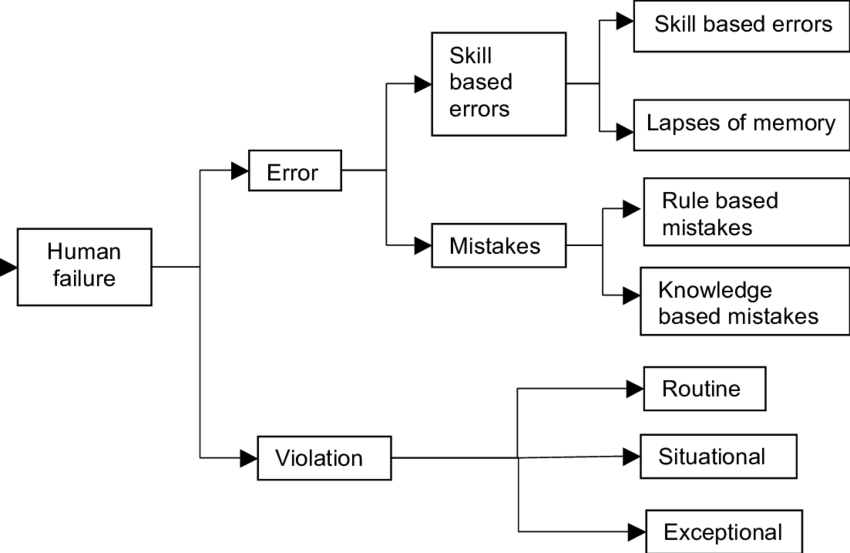
\includegraphics[width=0.7\textwidth]{types_of_human_failure.png} \footnote{\url{https://doi.org/10.21125/inted.2016.0391}}
\end{frame}
\note[itemize]{
    \item Skill based error (``slips'') - example: logic bug.  Hard to prevent other than over-practice.
    \item Lapses of memory (``lapses'') - example: syntax bug.  Use of checks such as CI, regression tests, linters.
    \item Mistakes - think you are doing the right thing, but it is the wrong thing.  Requires understanding of ``right'' to trap and mitigate.  Checklists and standards can help, but they need to be standard!
    \begin{itemize}
        \item Rule based mistakes
        \begin{itemize}
            \item You drive over the speed limit because you get where you are going faster, and you get a ticket - bad rule that usually works
            \item Incorrectly programmed a new infusion pump following the directions used for an older model and the pump failed - good rule in wrong situation
        \end{itemize}
        \item Knowledge based mistakes
        \begin{itemize}
            \item You apply an incorrect technique using concepts you aren't familiar with
            \item You misdiagnose a bug and take inappropriate action to correct it
            \item You react incorrectly to a bug based on an incomplete understanding of the system
        \end{itemize}
    \end{itemize}
    \item Routine violation - everyone is doing it, so I'll do it.  Example: speeding.
    \item Situation violation - need to do this to make progress.  Example: overriding GitHub merge requirements
    \item Exceptional violation - no thought or care for the consequences.
}
\begin{frame}{Addressing Human Error}
    Design systems where:
    \begin{itemize}
        \item Likelihood of making an error is reduced
        \item Motivation for making violations is reduced
        \item When failures occur, we can do something about it
    \end{itemize}
\end{frame}
\begin{frame}
    \begin{quote}
        Safety is not just the absence of accidents and incidents, but rather the presence of barriers and defenses and the capacity of the system to fail safely - Todd Conklin
    \end{quote}
\end{frame}
\begin{frame}{Normalization of Deviance}
    Why do violations occur?
    \begin{itemize}
        \item Always looking to be more efficient/effective
        \item Standards and best practices vs. efficiency and effectiveness
        \item Erosion of safety margins
        \item Most of the time, no adverse outcomes
    \end{itemize}
\end{frame}
\begin{frame}{How can we empower everyone to bring up errors?}
    Psychological Safety - a shared belief within the team that it is safe to take interpersonal risks
\end{frame}
\begin{frame}{Psychological Safety}
    \begin{itemize}
        \item Inclusion
        \item Learner Safety
        \item Contributor Safety
        \item Challenger Safety
    \end{itemize}
\end{frame}
\note[itemize]{
    \item Inclusion - make everyone feel welcome
    \item Learner Safety - normalize making mistakes, depersonalize feedback.  Focus on observable actions, not about individuals
    \item Contributor Safety - normalize different approaches and novel contributions.  Not ``we've always done it this way''
    \item Challenger Safety - normalize raising concerns.
    
    Leaders - ask for help, highlight own mistakes, be human
}
\begin{frame}{Just Culture}
    \begin{itemize}
        \item Everyone is fallible, errors will happen
        \item However, willful negligence still needs to be held to account
    \end{itemize}

    \begin{quote}
        [Just culture is] an atmosphere of trust in which people are encouraged (even rewarded) for providing essential information, but in which the line must be drawn between acceptable and unacceptable behavior.
    \end{quote}
\end{frame}
\begin{frame}{Just Culture}
    \begin{itemize}
        \item Context-rich stories
        \item Detailed analysis
        \item Evaluate rules
        \item Share learnings
        \item Apply rules in new situations
        \item Repeat
    \end{itemize}
\end{frame}
\begin{frame}{Just Culture in Medicine}
    \centering
    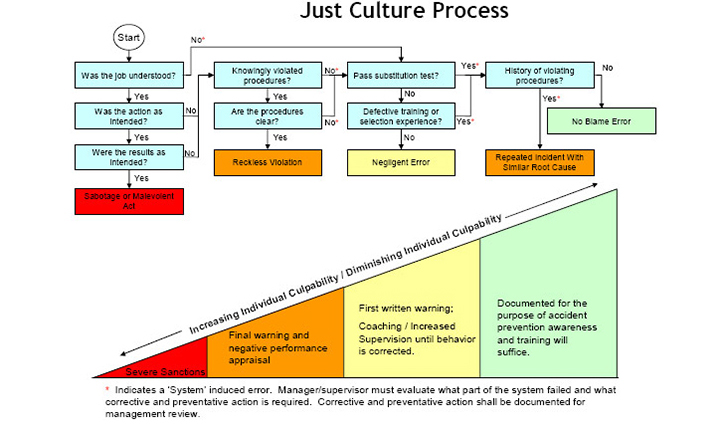
\includegraphics[width=0.7\textwidth]{just_culture_UA.jpg} \footnote{\url{https://deptmedicine.arizona.edu/patient-care/blog/quality-safety-\%E2\%80\%98just-culture\%E2\%80\%99-provides-process-review-correct-mistakes-optimal}}
\end{frame}
\begin{frame}{SRK Decision-Making Model}
    \centering
    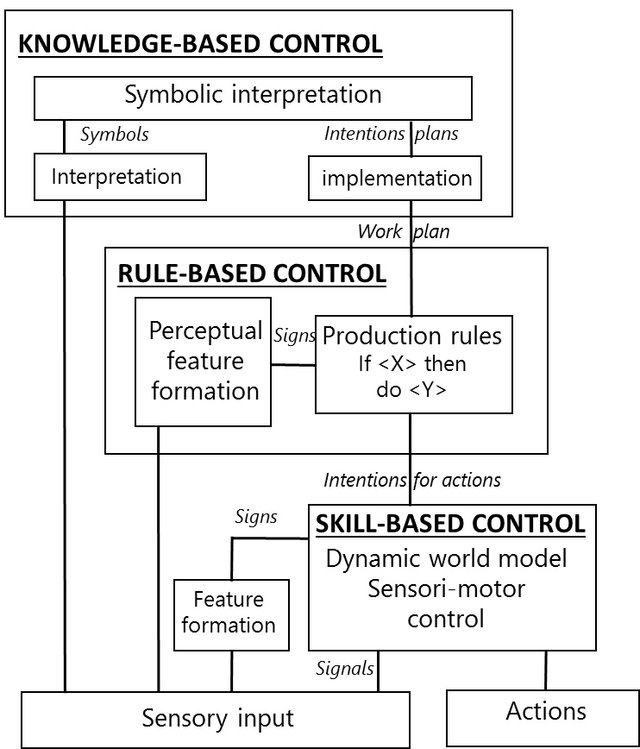
\includegraphics[height=0.75\textheight]{Rasmussen1989_SRK_model.jpg} \footnote{\url{http://dx.doi.org/10.3917/th.801.0007}}
\end{frame}
\begin{frame}{Sources of Errors}
    \begin{itemize}
        \item Skills-based errors - 1:10000
        \item Rules-based errors - 1:100
        \item Knowledge-based errors - 1:2
    \end{itemize}
\end{frame}
\note[itemize]{
    \item Skills-based - errors associated with distractions.  Improve through deliberate practice - perfect practice makes perfect.
    \item Rules-based - errors associated with applying wrong rule.  Improve through exposure to different situations with subtle differences to emphasize applicability of rules.
    \item Knowledge based - errors associated with lack of experience/knowledge.  Improve by providing method/philosophy of approaching problems.
}
\end{document}
